\section{Reduction to coupled first order differential equations}


The fundamental problem we wish to solve is to evolve the wave equation on Schwarzschild space-time with a source. However, to begin to address this problem, I implemented a one dimensional wave equation solver in C++ using the Discontinuous Galerkin method in flat space-time. The wave equation in flat space-time is given, in several different forms, by
\begin{eqnarray}
  \Box\psi=0\\
  \frac{\partial^2\psi}{\partial t^2}=\nabla\psi\\
  \frac{\partial^2\psi}{\partial t^2}=\frac{\partial^2 \psi}{\partial r^2}
\end{eqnarray}
where the final form is specialized to one dimension and $c=1$ in natural units. To numerically integrate this, it is necessary to reduce this second order differential equation to three coupled differential first order differential equations. There is a classical solution to this problem, which we follow. We introduce variables $\rho=\frac{\partial \psi}{\partial t}$ and $\phi = \frac{\partial\psi}{\partial r}$. With these definitions, and remembering that we want time evolution equations rather than spatial evolution equations, the three coupled equations become
\begin{eqnarray}
  \frac{\partial\psi}{\partial t} = \rho\nonumber\\
  \frac{\partial\rho}{\partial t} = \frac{\partial \phi}{\partial r}\nonumber\\
  \frac{\partial\phi}{\partial t} = \frac{\partial \rho}{\partial r}
  \label{stateev}
\end{eqnarray}
This system of equations can be rewritten
\begin{equation}
  \frac{\partial u}{\partial t} = A\frac{\partial u}{\partial r} + Bu\nonumber\\\
  \frac{\partial u}{\partial t} = RHS(u,t)
  \label{matrixdiff}
\end{equation}
where $u$ is the state vector consisting of $u=(\psi,\rho,\phi)$, and $A$ and $B$ are matrices. RHS stands for Right Hand Side. The C++ code has been implemented for wave equations of this generalized form, which encompasses wave equations on a Schwarzschild space-time.




\section{Spatial grids}
Our code solves a wave equation, which must first calculate a spatial derivative then integrate in time to solve a differential equation. For the spatial derivative part of the scheme, we make use of the Discontinuous Galerkin method to compute spatial derivatives, as a replacement for a finite difference scheme. Its has three primary benefits. One is that it naturally handles discontinuities in the evolved field, which is important to the effective source approach that we use when calculating orbits with a source in curved space-time. The second is that its accuracy scales exponentially with increasing polynomial order. 


\subsection{Finite difference schemes}
The classic solution to the spatial derivative problem is the finite difference scheme. In a one dimensional finite difference scheme, space is discretized into points on a line. The spatial derivative is calculated using a stencil of points that is symmetric about the point where one wants to know the spatial derivative, and extends $2n$ points beyond to either side, where $n$ is the order of the expansion. The spatial derivative is calculated from a weighted sum of the points included in the stencil, where some of the weights are negative. A stencil with $2n-1$ points in it, in one dimension, corresponds to an $n$th order expansion. It is possible to expand any order of derivative to any order of expansion. A first derivative, to second order accuracy, given by:
\begin{equation}
  D_r^{(2)}=\frac{1}{h}(-\frac{1}{2}f_{-1}+\frac{1}{2}f_1)
\end{equation}
Here the $f_{-1}$ and $f_1$ indicate the function evaluated at the grid point to either side of the $0$th grid point, where the derivative is evaluated. Here $h$ is the spacing between grid points. 
\begin{equation}
  D_r^{\prime (2)}=\frac{1}{h^2}(f_{-1}-2f_0+f_1)
\end{equation}

It is possible to extend these stencils to two and three dimensions. When considering parallelization using OpenMP, issues of synchronization must be considered. When parallelizing over many nodes, the spatial grid gets divided into blocks. At the ends of each block, the boundary cells need information from the neighboring cells to calculate the spatial derivative. For an order $n$ derivative, $n-1$ boundary cells are synchronized into buffer zones both to the left and to the right at each time step. In our code, this is not necessary, since we have parallelized with OpenMP, which uses shared memory within one node, across several (16) cores.

\subsection{The Discontinuous Galerkin method}
The Discontinuous Galerkin method breaks space into segments called elements. Within each element, the value of the field is represented by the sum of $n+1$ interpolating polynomials of order $n$, where $n$ is the order of the element. There are $n+1$ unevenly spaced nodes in the element, clustered toward the edges. At each node, exactly one of the interpolating polynomials takes on a value of one while the others are zero. An interpolating Lagrange polynomial has a functional form:
\begin{equation}
  \ell_i(r)=\prod_{j=1,j\ne i}^{n}\frac{r-\xi_j}{\xi_i-\xi_j}
\end{equation}
where $\xi_i$ is a location of a node and where $r$ is an arbitrary position~\cite{dghesthaven}. 


Omitting the details of the derivation of this method, which can be found in Reference~\cite{dghesthaven}, the procedure for calculating the spatial derivative in one dimension is to first calculate the Legendre polynomials. A matrix inversion is involved to calculate the derivative matrices, for which we use custom packages, the Template Numerical Toolkit and JAMA. It was discovered, upon parallelization with OpenMP, that TNT is not threadsafe. I rewrote most, but not all, of the code to avoid this issue; however, it would be better to replace TNT altogether if this code were developed further.

The Discontinuous Galerkin method helps damp error introduced by discontinuities in the field, provided they remain at element boundaries. We make use of this in our self-force calculations in the neighborhood of the particle, to be described in Chapter~\ref{ellipticalorb}. The numerical flux how information passes from one element to the next in the Discontinuous Galerkin method and is a way of accounting for the discontinuity in the flow between neighboring elements. The specific method we use for calculating the numerical flux breaks breaks the wave velocities into in-going and outgoing components. At each element boundary, the state vector from external to the element is coupled to the in-going velocity then added to the state vector internal to the element coupled to the outgoing velocity. The contribution from each boundary is distributed across the element according to a lift matrix. This is repeated at each time step. Discontinuities can exist at the boundaries, but not within an element. 



\section{Time evolution}

Time evolution in our code is handled by a fourth order low storage Runga Kutta method. Instead of the standard fourth order Runga Kutta method, this method takes five sub-time-steps, but only the most recent sub-time-step needs to be stored.

\begin{eqnarray}
  p^{(0)}=&u^n\nonumber\\
  k^{(i)}=&a_ik^{(i-1)}+\delta t RHS(p^{(i-1)},t^n+c_i\delta t)\nonumber\\
  p^{(i)}=&p^{(i-1)}+b_iK^{(i)}\nonumber\\
  u_h^{n+1}=&p^{(5)}
\end{eqnarray}
Here steps two and three are repeated for $i=1-5$, first $k$, then $p$, then increase $i$ and repeat. The coefficients $a_i$, $b_i$, and $c_i$ are given in Reference~\cite{dghesthaven}.

\section{Wave equation on flat space-time}

Using Gaussian initial conditions in $\psi$ and setting the $\rho$ (Equation~\ref{statev}) initial conditions to the derivative of that Gaussian, I have produced the evolution shown in Figure~\ref{gaussWave}. The Gaussian splits into two, evolves both left and right, hits the periodic boundary conditions, and re-enters the one-dimensional space on the opposite side, eventually returning to its original position and re-merging. A progression from left to right can be seen in Figure~\ref{sineWave} for sinusoidal initial conditions with a sinusoidal initial condition in $\psi$ and cosine initial conditions in $\phi$ (Equation~\ref{stateev}). Again, periodic boundary conditions cause the wave to cross to the opposite side and re-enter.

\begin{figure}
  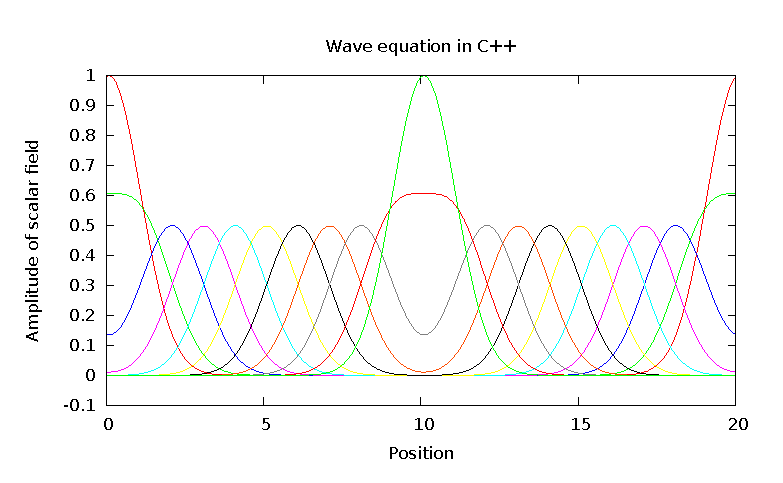
\includegraphics{gaussWave}
  \caption{Waves evolving over time for Gaussian initial conditions}
  \label{gaussWave}
\end{figure}

\begin{figure}
  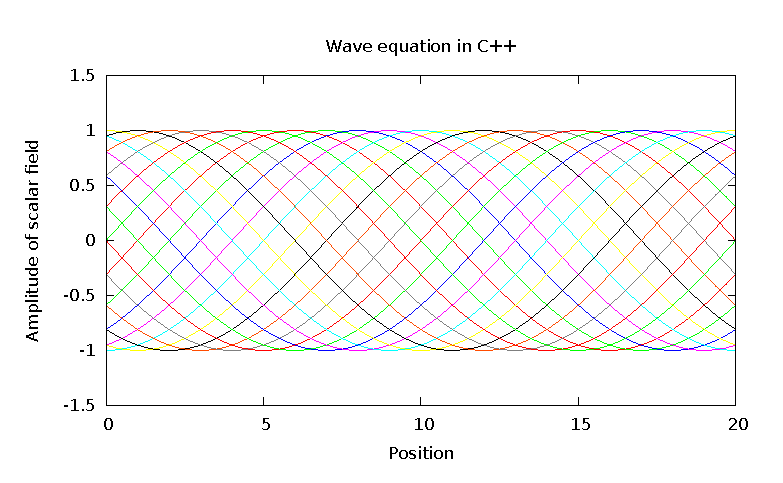
\includegraphics{sineWave}
  \caption{Waves evolving over time for sinusoidal initial conditions}
  \label{sineWave}
\end{figure}

The Discontinuous Galerkin method has truncation error that scales as $h^{n+1}$, where $h$ is the element size and $n$ is the polynomial order of the elements. The $L_2$ error is defined as the square root of the sum of the squared differences across all space, after one complete cycle of the system. Because of the periodic boundary conditions, the system should be the same after one complete cycle, making a meaningful error estimate possible. The scaling of the $L_2$ error with DG order and with element size is shown in Figures~\ref{scalingorder} and~\ref{scalingelement}. The scaling matches expectations until roundoff error is hit, where the error stops improving with order or smaller element size. Not shown, this same pattern was seen for the $L_0$ error, which is the maximum error over all space.

\begin{figure}
  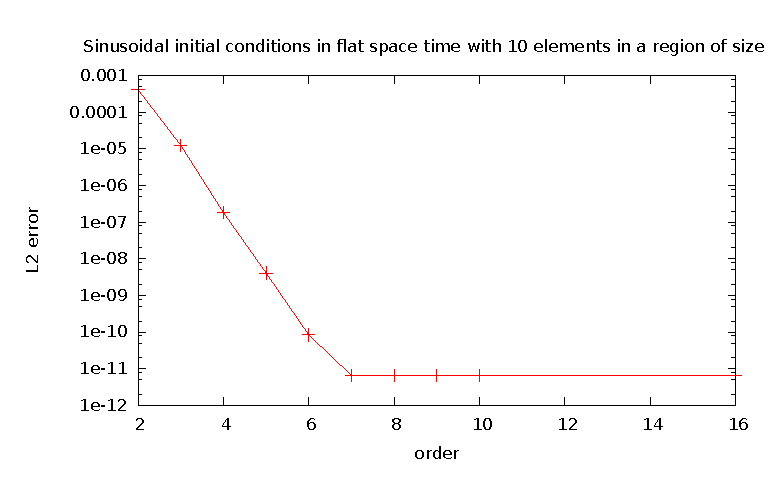
\includegraphics{sinL2WTorder}
  \caption{$L_2$ error scaling with DG order for sinusoidal initial conditions with ten elements with element size $h=0.01$.}
  \label{scalingorder}
\end{figure}

\begin{figure}
  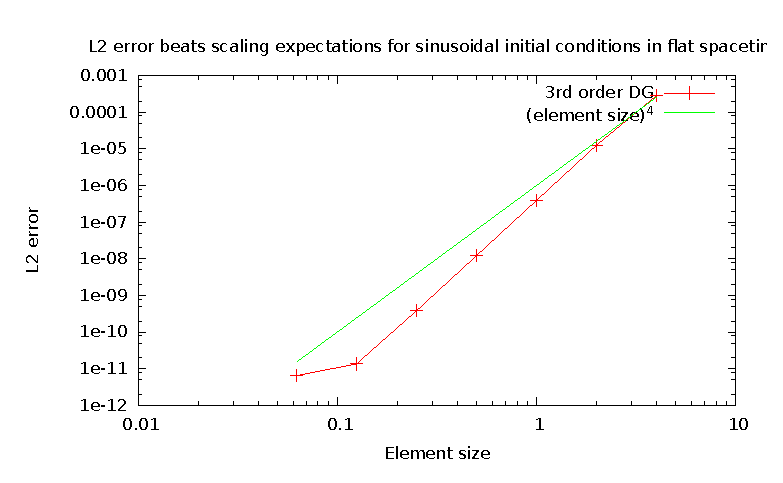
\includegraphics{sinL2WTelement}
  \caption{$L_2$ error scaling with element size for sinusoidal initial conditions. The error seems to be super-convergent. This requires cancellations due to symmetry, perhaps due to the symmetry of wave propagation speed in either direction in flat spacetime.}
  \label{scalingelement}
\end{figure}


